% Vortragsinhalt  „Vom Skalarprodukt zur Bildbearbeitung”

% Definitionen/Pakete für Handout und Aufgaben

\KOMAoptions{parskip=half, headinclude=true, headsepline=true}

% Pakete
\usepackage{fontspec}
\setmainfont{Latin Modern Roman}
\usepackage[ngerman]{babel}
\usepackage{csquotes}
\usepackage{graphicx}
\newcommand*{\imagesourcefolder}{./Bilder}
\graphicspath{{\imagesourcefolder/}}
\usepackage{xcolor}
\usepackage{wrapfig}
\usepackage{mathtools}
\usepackage[per-mode=fraction]{siunitx}
\usepackage{tikz,pgfplots}
\usepgfplotslibrary{polar}
\usetikzlibrary{arrows.meta}
\usetikzlibrary{plotmarks}
\usetikzlibrary{calc}
\pgfplotsset{compat=newest}
\usepackage{tabularx}
\usepackage{booktabs}

% Layout
\usepackage[
origlayout=true, automark, colors={mat},
headsepline=4pt,
intern  % spare Tinte
]{URpagestyles}
\pagestyle{URheadings}
\renewcommand{\titlepagestyle}{URtitle}
\addtokomafont{section}{\Large\normalfont\bfseries}

% Lückentext/Antworten
\usepackage[thickness=0pt,textcolor=gray]{cloze}
\clozesetfont{\LARGE\itshape}
\makeatletter
\newif\ifhide
\@ifclasswith{scrartcl}{hide}{\hidetrue}{\hidefalse}
\makeatother
\newcommand{\Loesung}[1]{\ifhide\relax\else{\clozefont{}\color{gray}#1}\fi}
\newcommand{\ausfuelltext}[1]{\cloze{#1\strut}}
\newcommand{\formel}[1]{\fcolorbox{gray}{white}{#1}}
\newcommand{\canvas}[3][c]{
  \parbox[#1]{#2}{~\\[-\baselineskip]%
    \formel{#3}%
    \\\hbox{}
  }
}

% Titel, Metadaten
\usepackage[colorlinks=true, linkcolor=blue,
pdfauthor={Gesina Schwalbe}
]{hyperref}
%\subject{Schülerzirkel am XX.XX.2018}
\date{}
\author{Gesina Schwalbe}



% Titel, Metadaten
\hypersetup{pdftitle={Vom Skalarprodukt zur Bildbearbeitung}}
\title{Vom Skalarprodukt zur Bildbearbeitung}
\ohead{Vom Skalarprodukt zur Bildbearbeitung}


\begin{document}
\maketitle

\section*{Definitionen}
\textbf{Vektor\strut} \enquote{Wegbeschreibung}

\begin{tabularx}{1.1\linewidth}{@{} X r @{}}
  \begin{minipage}[t]{\linewidth}
    \textbf{Koordinatensystem}\par
    \begin{enumerate}
    \item \ausfuelltext{Nullpunkt}
    \item \ausfuelltext{Grundrichtungen mit (Schritt)\-Län\-gen in best. Reihenfolge}
      \\so, dass:
      \begin{itemize}
      \item \ausfuelltext{Jeder Punkt erreichbar}
      \item \ausfuelltext{So wenige wie möglich}
      \end{itemize}
    \end{enumerate}
  \end{minipage}
  & \canvas[t]{0.5\linewidth}{
    \ausfuelltext{% Beispiel für ein Koordinatensystem mit einem Beispielvektor

\begin{tikzpicture}
  \begin{axis}[
    width=\linewidth,
    font=\scriptsize,
    axis equal, axis lines=center,
    xticklabels=\empty, yticklabels=\empty,
    xmin=-2.5, xmax=2.5, xtick distance=1,% minor x tick num=1,
    ymin=-2.5, ymax=2.5, ytick distance=1,% minor y tick num=1
    grid=major
    ]
    \coordinate (0) at (axis cs:0,0);
    \draw[fill] (0) circle[radius=2pt];
    \draw[thick, -Stealth] (0) -- (axis cs:1,0)
    node [pos=1, below] {$(1,0)$};
    \draw[thick, -Stealth] (0) -- (axis cs:0,1)
    node [pos=1, left] {$(0,1)$};
    
    \draw[-Stealth] (axis cs:1,0) -- (axis cs:2,0);
    \draw[-Stealth] (axis cs:2,0) -- (axis cs:2,1);
    % \draw[-Stealth] (axis cs:2,1) -- (axis cs:2,2);

    \coordinate (ex) at (axis direction cs:2,1);
    \coordinate (other) at (axis cs:-2.5,-1.5);
    \draw[thick, -Stealth] (0) -- ($(0)+(ex)$)
    node [pos=1, left] {$(2,1)$};
    \draw[thick, -Stealth] (other)  -- ($(other)+(ex)$)
    node [pos=1, left] {$(2,1)$};
  \end{axis}
\end{tikzpicture}
}}
\end{tabularx}

\textbf{Vektordarstellung}\par
    \formel{\ausfuelltext{
        $\Big(
        \text{<Schritte in Richtung 1>},
        \text{<Schritte in Richtung 2>},
        \dots
        \Big)$
      }}
\ifhide\relax\else{
  \begin{itemize}
  \item Die Reihenfolge, in der ich die Schritte mache, ist egal!
  \item Auch Schrittbruchteile sind erlaubt.
  \end{itemize}
}\fi

\section*{Rechnen mit Vektoren}
\begin{tabularx}{1.15\linewidth}{@{} X l @{}}
  \textbf{Addition\strut}\par
  \formel{$(x_1,\dots,x_n) + (y_1,\dots,y_n) =
    \text{\ausfuelltext{$(x_1+y_1,\dots,x_n+y_n)$}}$}
  \par
  Beispiel: $(2,1) + (-1,1) = \text{\ausfuelltext{$(1,2)$}}$
  & \canvas[t]{0.35\linewidth}{% Beispiel einer Vektoraddition

\begin{tikzpicture}
  \begin{axis}[
    width=\linewidth,
    font=\scriptsize,
    axis equal, axis lines=center,
    xmin=0, xmax=2.1, xtick distance=1, xticklabels=\empty,
    ymin=0, ymax=2.1, ytick distance=1, yticklabels=\empty
    ]
    \coordinate (A) at (axis cs:0,0);
    \coordinate (B) at (axis cs:2,1);
    \coordinate (C) at (axis cs:1,2);
    \draw[thick, -Stealth] (A) -- (B)
    node [pos=0.75,below] {$(2,1)$};
    \draw[thick, -Stealth] (B) -- (C)
    node [pos=0.75,right] {$(-1,1)$};
    \draw[thick, -Stealth] (A) -- (C)
    node [pos=0.75,left] {$(1,2)$};
  \end{axis}
\end{tikzpicture}}\\
  \textbf{Strecken/Stauchen\strut}\par
  \formel{$(x_1,\dots,x_n) + (y_1,\dots,y_n) =
    \text{\ausfuelltext{$(a\cdot x_1,\dots,a\cdot x_n)$}}$}
  \par
  Beispiel: $\frac 12 \cdot (2,1) = \text{\ausfuelltext{$(1,\frac 12)$}}$
  & \canvas[t]{0.35\linewidth}{\begin{tikzpicture}
  \begin{axis}[
    width=\linewidth,
    font=\scriptsize,
    axis equal, axis lines=center,
    xticklabels=\empty, yticklabels=\empty,
    xmin=0, xmax=2.1, xtick distance=1, minor x tick num=1,
    ymin=0, ymax=1.1, ytick distance=1, minor y tick num=1
    ]
    \coordinate (A) at (axis cs:0,0);
    \coordinate (B) at (axis cs:2,1);
    \coordinate (C) at (axis cs:1,0.5);
    \draw[-Stealth] (A) -- (B)
    node [pos=0.9,below] {$(2,1)$};
    \draw[thick, -Stealth] (A) -- (C)
    node [pos=0.5,above] {$(1,\frac 1 2)$};
  \end{axis}
\end{tikzpicture}}
\end{tabularx}
Insbes. \formel{$(x_1,\dots,x_n) =
  x_1\cdot(1,0,\dotsc,0) +
  x_2\cdot(0,1,0,\dotsc) + \dotsb +
  x_n\cdot(0,\dotsc,0,1)
  $}


\section*{Andere Räume mit Koordinatensystem}
\begin{itemize}
\item RGB-Farbpixel: (Rotwert, Grünwert, Blauwert)
\item Schwarz-weiß Bild: (Helligkeit Pixel 1, Helligkeit Pixel 2,
  \dots)
  \hfill
  \parbox[b][1eM]{6em}{\frame{
\includegraphics[width=6em]{bildvektor}}}
\end{itemize}


\section*{Skalarprodukt}
\begin{wrapfigure}[5]{r}{0.3\linewidth}
  \begin{tikzpicture}
  \pgfplotsset{
    every axis plot post/.style={solid, thick, mark=*}}
  \begin{axis}[
    font=\scriptsize,
    width=1.75\linewidth,
    axis equal,
    axis lines=middle,
    xmin=-1.2, xmax=1.2, xtick distance=0.5, ticklabel style={font=\tiny},
    ymin=-1.2, ymax=1.2, ytick distance=0.5,
    ]
    \begin{scope}[every node/.style={pos=1, black}]
      \addplot[gray] coordinates {(0,0) ({1/sqrt(2)},{1/sqrt(2)})}
      node[above] {$\frac{1}{\sqrt{2}}(1,1)$};
      \addplot[gray] coordinates {(0,0) (0,1)}
      node[above right] {$(0,1)$};
      \addplot[gray] coordinates {(0,0) ({-1/sqrt(2)},{1/sqrt(2)})}
      node[above] {$\frac{1}{\sqrt{2}}(-1,1)$};
      \addplot[gray] coordinates {(0,0) (-1,0)}
      node[above left, xshift=0.5em] {$(-1,0)$};
      \addplot[gray] coordinates {(0,0) ({-1/sqrt(2)},{-1/sqrt(2)})}
      node[below] {$\frac{1}{\sqrt{2}}(-1,-1)$};
      \addplot[gray] coordinates {(0,0) (0,-1)}
      node[below right] {$(0,-1)$};
      \addplot[gray] coordinates {(0,0) ({1/sqrt(2)},{-1/sqrt(2)})}
      node[below,xshift=0.5em] {$\frac{1}{\sqrt{2}}(1,-1)$};
      \addplot[black,thick] coordinates {(0,0) (1,0)}
      node[above right] {$(1,0)$};
    \end{scope}
    \draw[gray!30, dashed] (axis cs:0,0) circle[radius=1];
  \end{axis}
\end{tikzpicture}
\end{wrapfigure}
\formel{$(x_1, \dotsc,x_n) \circ (y_1,\dotsc, y_n) =
  \text{\ausfuelltext{$x_1\cdot y_1 + x_2\cdot y_2 + \dotsb + x_n\cdot y_n$}}
  $}
Das Skalarprodukt ist ein Maß dafür,
\ausfuelltext{wie sehr zwei Vektoren in dieselbe Richtung
  zeigen.}

Genauer:\par
\formel{$x\circ y =
  \text{\ausfuelltext{$\text{Länge}(x) \cdot \text{Länge}(y) \cdot \cos(\phi)$}}$}

\bigskip
\bigskip
\begin{tikzpicture}
  \begin{axis}[
    width=\linewidth,
    height=0.5\linewidth,
    grid=both,
    grid style={dashed,gray!30},
    legend pos=south east,
    % 
    xlabel={$\text{Winkel $\phi$ zwischen (1,0) und $x$}$},
    axis x line=middle,
    xmin=0, xmax=380, xtick distance=90, minor x tick num=1,
    xticklabel={$\pgfmathprintnumber{\tick}\si{\degree}$},
    % 
    ylabel={$(1,0)\circ x$},
    axis y line=left,
    ymin=-1.1, ymax=1.1,
    ytick distance=0.5,
    extra y ticks={{-1/sqrt(2)},{1/sqrt(2)}},
    extra y tick labels={$-\frac{1}{\sqrt{2}}$,$-\frac{1}{\sqrt{2}}$},
    ]
    \ifhide\relax
    \else{
      \addplot[smooth,domain=0:360,samples=33,mark repeat=4,mark=o, mark color=gray] {cos(x)};
      \legend{$\cos(x)$}
    }
    \fi
  \end{axis}
\end{tikzpicture}


\section*{Anwendung in der Bildverarbeitung: Faltung}
Eine Faltung sammelt die Ergebnisse von Skalarprodukten eines
Vergleichsbildausschnitts mit Bildausschnitten unseres Anfangsbildes
in einem Ergebnisbild.
\begin{center}
  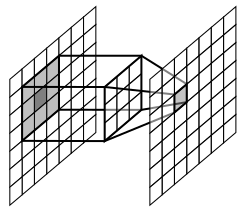
\includegraphics[width=0.5\linewidth]{faltung}
\end{center}

\begin{tabularx}{0.9\linewidth}{@{} X l @{}}
  \textbf{Wirkung der Faltung} & \textbf{Vergleichsbildausschnitt}\\\toprule
  horizontale (scharfe) Linie
  & \parbox[c]{4em}{
\includegraphics[width=\linewidth]{horizontale_linie-kern}}
  \\\midrule
  vertikale Kante von dunkel zu hell
  & \parbox[c]{4em}{
\includegraphics[width=\linewidth]{vertikale_kante-dunkel-kern}}
    \quad oder \quad
    \parbox[c]{4em}{
\includegraphics[width=\linewidth]{vertikale_kante-hell-kern}}
    \\\midrule
  Relief
  & \parbox[c]{4em}{
\includegraphics[width=\linewidth]{relief-kern}}
  \\\midrule
  Schärfen
  & \parbox[c]{4em}{
\includegraphics[width=\linewidth]{schaerfen-kern}}
  \\\bottomrule
\end{tabularx}

\subsection*{Beachte für den Umgang mit Bildern und Faltungen:}
\begin{itemize}
\item Pixelwerte
  $\begin{cases}
    <0 & \text{keine Farbe (schwarz)} \\
    >255 & \text{volle Farbe (weiß)} \\
  \end{cases}$
\item Für Vergleichsbildausschnitte sollte man beachten:
  \begin{itemize}
  \item Die Summe der Einträge sollte zwischen 0 und 1 sein.
  \item Um obige Bedingungen zu erreichen:
    Die Tendenz (hell zu dunkel) ist entscheidend.
  \end{itemize}
\end{itemize}

\enlargethispage{2cm}
\subsection*{Gimp Bedienung}
\begin{tabularx}{1.1\linewidth}{ @{} X l @{}}
  \texttt{Filters $\rightarrow$ Generic $\rightarrow$ Convolution
    Matrix…}
  \par
  Starte mit folgenden Einstellungen:
  &
  \parbox[t]{0.45\linewidth}{
    \vspace*{-3\baselineskip}
    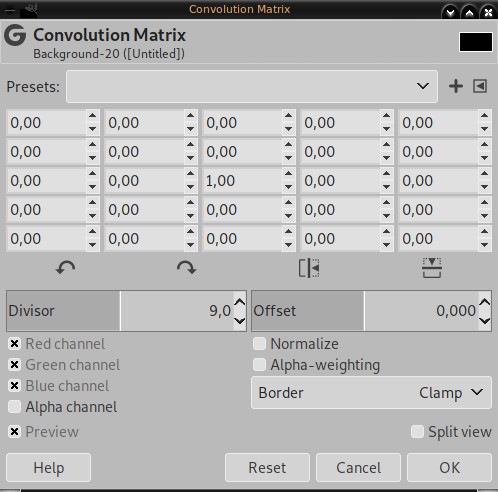
\includegraphics[width=\linewidth]{faltung_gimp_screenshot}
  }
\end{tabularx}
\end{document}
